\documentclass[aspectratio=169,usenames,dvipsnames,pdftex]{beamer}

\usepackage{listings}
\usepackage{xcolor}
\usepackage{multicol}
\usepackage{media9}
\usepackage{siunitx}
\usepackage[scale=2]{ccicons}
% Glyphs
\usepackage{fontawesome5}

\usepackage{booktabs}
\usepackage{appendixnumberbeamer}
\usepackage{csquotes}

\usepackage{pgfplots}
\usepgfplotslibrary{dateplot}

\usepackage{tikz}
\usetikzlibrary[topaths]
\usepackage{xspace}

\usetikzlibrary{shapes,snakes}
\usepackage{amsmath,amssymb}

%%%%%%%%%%%%%%%%
%% Title Page %%
%%%%%%%%%%%%%%%%
\title{GNU Emacs}
\subtitle{\texttt{The True Text Editor}}
\date{\today}
\author{Abd El-Twab M. Fakhry}
\institute{Free Software Foundation}
\titlegraphic{\hfill\includegraphics[height=1.5cm]{Emacs-Logo.png}}

%%%%%%%%%%%%%%%%%%%
%% Common colors %%
%%%%%%%%%%%%%%%%%%%
\definecolor{charcoal}{rgb}{0.21, 0.27, 0.31}
\definecolor{champagne}{rgb}{0.97, 0.91, 0.81}
\definecolor{dimgray}{rgb}{0.41, 0.41, 0.41}
\definecolor{flax}{rgb}{0.93, 0.86, 0.51}
%% Code colors
\definecolor{lavendergray}{rgb}{0.77, 0.76, 0.82}
\definecolor{lightslategray}{rgb}{0.47, 0.53, 0.6}
\definecolor{egyptianblue}{rgb}{0.06, 0.2, 0.65}
\definecolor{ballblue}{rgb}{0.13, 0.67, 0.8}
\definecolor{greencssgreen}{rgb}{0.0, 0.5, 0.0}
\definecolor{eggshell}{rgb}{0.94, 0.92, 0.84}
\definecolor{lava}{rgb}{0.81, 0.06, 0.13}
\definecolor{lavenderindigo}{rgb}{0.58, 0.34, 0.92}
\definecolor{mediumred-violet}{rgb}{0.73, 0.2, 0.52}
\definecolor{black}{rgb}{0.0, 0.0, 0.0}
\definecolor{forestgreen}{rgb}{0.13, 0.55, 0.13}
\definecolor{harvardcrimson}{rgb}{0.79, 0.0, 0.09}

%%%%%%%%%%%%%%%%%%%%%%%%%
%% Syntax Highlighting %%
%%%%%%%%%%%%%%%%%%%%%%%%%
\input{syntax.tex}

%%%%%%%%%%%
%% Theme %%
%%%%%%%%%%%
\usetheme[
progressbar=frametitle,
titleformat=smallcaps,
numbering=fraction,
block=fill,
background=light
]{metropolis}

\useoutertheme{metropolis}
\useinnertheme{metropolis}
\usefonttheme{metropolis}
\usecolortheme{seahorse}
\setbeamercolor{background canvas}{bg=champagne}
\setbeamercovered{transparent=5}

%%%%%%%%%%%%%%%%%%%%%%
%% Global Variables %%
%%%%%%%%%%%%%%%%%%%%%%
\newcommand{\themename}{\textbf{\textsc{Metropolis}}\xspace}
\newcount\mycount

%%%%%%%%%%%%%%%%%%%%
%% Document Start %%
%%%%%%%%%%%%%%%%%%%%
\begin{document}

	\maketitle

	\begin{frame}{Table of contents}
		\setbeamertemplate{section in toc}[sections numbered]
		\tableofcontents[hideallsubsections]
	\end{frame}

  \section{Code}

  \begin{frame}[allowframebreaks, containsverbatim]{Code}
    \lstinputlisting[style=solidity]{simple-auction.sol}
  \end{frame}

	\section{Introduction}

	\begin{frame}[fragile]{Metropolis}
		\begin{verbatim}\documentclass{beamer}
		\usetheme{metropolis}\end{verbatim}
	\end{frame}

	\begin{frame}[fragile]{Sections}
		Sections group slides of the same topic
		\begin{verbatim}\section{Elements}\end{verbatim}
	\end{frame}

	\section{Title formats}

	\begin{frame}{Metropolis title formats}
		\themename supports 4 different title formats:
		\begin{itemize}
			\item Regular
			\item \textsc{Small caps}
			\item \textsc{all small caps}
			\item ALL CAPS
		\end{itemize}
		They can either be set at once for every title type or individually.
	\end{frame}

	{
		\metroset{titleformat frame=smallcaps}
		\begin{frame}{Small caps}
			This frame uses the \textsc{Smallcaps} title format.

			\begin{alertblock}{Potential Problems}
				Be aware that not every font supports small caps.
        If for example you typeset your presentation with pdfTeX and the Computer Modern Sans Serif font, every text in small caps will be typeset with the Computer Modern Serif font instead.
			\end{alertblock}
		\end{frame}
	}

	{
		\metroset{titleformat frame=allsmallcaps}
		\begin{frame}{All small caps}
			This frame uses the \texttt{allsmallcaps} title format.

			\begin{alertblock}{Potential problems}
				As this title format also uses small caps you face the same problems as with the \texttt{smallcaps} title format. Additionally this format can cause some other problems. Please refer to the documentation if you consider using it.

				As a rule of thumb: just use it for plaintext-only titles.
			\end{alertblock}
		\end{frame}
	}

	{
		\metroset{titleformat frame=allcaps}
		\begin{frame}{All caps}
			This frame uses the \texttt{allcaps} title format.

			\begin{alertblock}{Potential Problems}
				This title format is not as problematic as the \texttt{allsmallcaps} format, but basically suffers from the same deficiencies. So please have a look at the documentation if you want to use it.
			\end{alertblock}
		\end{frame}
	}

	\section{Elements}

	\begin{frame}[fragile]{Typography}
		\begin{verbatim}The theme provides sensible defaults to
		\emph{emphasize} text, \alert{accent} parts
		or show \textbf{bold} results.\end{verbatim}

		\begin{center}becomes\end{center}

		The theme provides sensible defaults to \emph{emphasize} text,
		\alert{accent} parts or show \textbf{bold} results.
	\end{frame}

	\begin{frame}{Font feature test}
		\begin{itemize}
			\item Regular
			\item \textit{Italic}
			\item \textsc{Small Caps}
			\item \textbf{Bold}
			\item \textbf{\textit{Bold Italic}}
			\item \textbf{\textsc{Bold Small Caps}}
			\item \texttt{Monospace}
			\item \texttt{\textit{Monospace Italic}}
			\item \texttt{\textbf{Monospace Bold}}
			\item \texttt{\textbf{\textit{Monospace Bold Italic}}}
		\end{itemize}
	\end{frame}

	\begin{frame}{Lists}
		\begin{columns}[T, onlytextwidth]
			\column{0.20\textwidth}
				Items
				\begin{itemize}
					\item Milk \item Eggs \item Potatoes
				\end{itemize}

			\column{0.23\textwidth}
				Enumerations 1.
				\begin{enumerate}
					\item First, \item Second and \item Last.
				\end{enumerate}

			\column{0.23\textwidth}
				Enumerations A.
				\begin{enumerate}[A.]
					\item First, \item Second and \item Last.
				\end{enumerate}

			\column{0.28\textwidth}
				Descriptions
				\begin{description}
					\item[PowerPoint] Meeh. \item[Beamer] Yeeeha. \item[Google] Naah.
				\end{description}
		\end{columns}
	\end{frame}

	\begin{frame}{Animation}
		\begin{itemize}[<+- | alert@+>]
			\item \textbf<4,5>{\alert<4,5>{This is\only<4,5>{ really} important}}
			\item \only<2,3,4>{Now this}\only<5>{\textcolor{magenta}{I Love You \faHeart}}
			\item And now this
		\end{itemize}
	\end{frame}

	\begin{frame}{Figures}
		\begin{figure}
      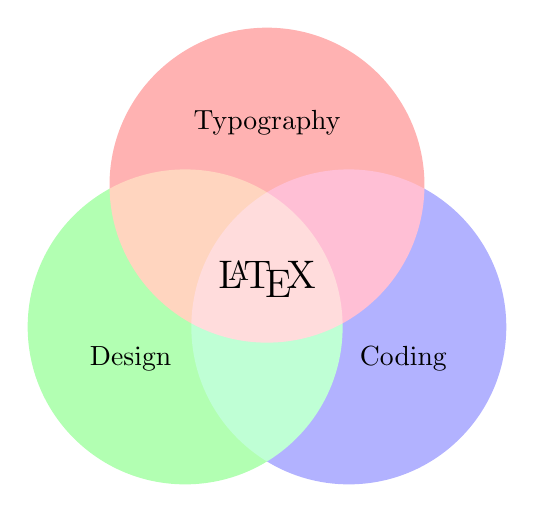
\begin{tikzpicture}
        \begin{scope}[blend group = soft light]
          \fill[red!30!white]   ( 90:1.2) circle (2);
          \fill[green!30!white] (210:1.2) circle (2);
          \fill[blue!30!white]  (330:1.2) circle (2);
        \end{scope}
        \node at ( 90:2)    {Typography};
        \node at ( 210:2)   {Design};
        \node at ( 330:2)   {Coding};
        \node [font=\Large] {\LaTeX};
      \end{tikzpicture}
      \caption{A Venn diagram from
			\href{http://www.texample.net/tikz/examples/rotated-polygons/}{texample.net}.}
		\end{figure}
	\end{frame}

  \begin{frame}{Graphs}
    \begin{figure}[htb]
      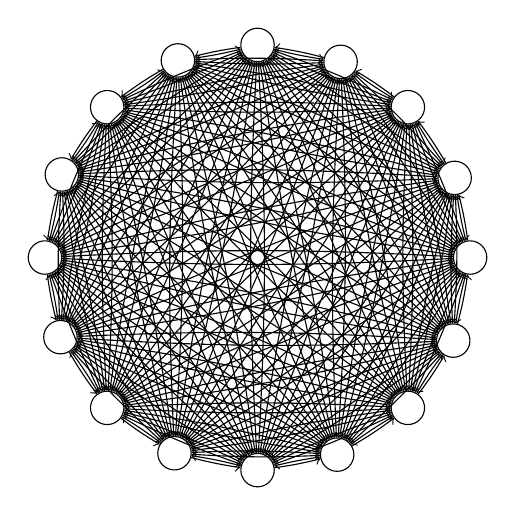
\begin{tikzpicture}[transform shape]
        \foreach \number in {1,...,8}{
        	\mycount=\number
        	\advance\mycount by -1
        	\multiply\mycount by 45
        	\advance\mycount by 0
          \node[draw,circle,inner sep=0.15cm] (N-\number) at (\the\mycount:2.7cm) {};
        }
        \foreach \number in {9,...,16}{
          \mycount=\number
        	\advance\mycount by -1
        	\multiply\mycount by 45
          \advance\mycount by 22.5
          \node[draw,circle,inner sep=0.15cm] (N-\number) at (\the\mycount:2.7cm) {};
        }
        \foreach \number in {1,...,15}{
        	\mycount=\number
        	\advance\mycount by 1
        	\foreach \numbera in {\the\mycount,...,16}{
          	\path (N-\number) edge[->,bend right=3] (N-\numbera)  edge[<-,bend left=3] (N-\numbera);
        	}
      	}
      \end{tikzpicture}
      \caption{Complete graph from
			\href{https://texample.net/tikz/examples/complete-graph/}{texample.net}.}
    \end{figure}
  \end{frame}

	\begin{frame}{Tables}
		\begin{table}
			\caption{Largest cities in the world (source: Wikipedia)}
			\begin{tabular}{@{} llr @{}}
				\toprule
				City & Country & Population\\
				\midrule
				Tokyo & Japan & 37,400,068\\
				Delhi & India & 28,514,000\\
				Shanghai & China & 25,582,000\\
				São Paulo & Brazil & 21,650,000\\
				Mexico City & Mexico & 	21,581,000\\
				Cairo & Egypt & 20,076,000\\
				\bottomrule
			\end{tabular}
		\end{table}
	\end{frame}

	\begin{frame}{Blocks}
		Three different block environments are pre-defined and may be styled with an
		optional background color.

		\begin{columns}[T,onlytextwidth]
			\column{0.95\textwidth}
				\begin{block}{Default}
					Block content.
				\end{block}

				\begin{alertblock}{Alert}
					Block content.
				\end{alertblock}

				\begin{exampleblock}{Example}
					Block content.
				\end{exampleblock}
		\end{columns}
	\end{frame}

	\begin{frame}{Math}
    \begin{equation*}
      \phi(ab) = \phi(a) \cdot \phi(b) \cdot \frac{d}{\phi(d)}
    \end{equation*}
	\end{frame}

	\begin{frame}{Line plots}
		\begin{figure}
			\begin{tikzpicture}
				\begin{axis}[
					mlineplot,
					width=0.9\textwidth,
					height=6cm,
          xlabel={x},
          ylabel={y},
				]
					\addplot {sin(deg(x))};
					\addplot+[samples=100] {cos(deg(x))};
          \legend{sin(x), cos(x)}
				\end{axis}
			\end{tikzpicture}
		\end{figure}
	\end{frame}

	\begin{frame}{Bar charts}
		\begin{figure}
			\begin{tikzpicture}
				\begin{axis}[
					mbarplot,
					xlabel={Foo},
					ylabel={Bar},
					width=0.9\textwidth,
					height=6cm,
				]
				\addplot plot coordinates {(1, 20) (2, 25) (3, 22.4) (4, 12.4)};
				\addplot plot coordinates {(1, 18) (2, 24) (3, 23.5) (4, 13.2)};
				\addplot plot coordinates {(1, 10) (2, 19) (3, 25) (4, 15.2)};
				\legend{lorem, ipsum, dolor}
				\end{axis}
			\end{tikzpicture}
		\end{figure}
	\end{frame}

	\begin{frame}{Quotes}
		\begin{quote}
      My general working style is to write everything first with pencil and paper, sitting beside a big wastebasket. Then I use Emacs to enter the text into my machine.
      \begin{center}— Donald E. Knuth\end{center}
		\end{quote}
	\end{frame}

	{
		\setbeamertemplate{frame footer}{By: AbdeltwabMF}
		\begin{frame}[fragile]{Frame footer}
			\themename defines a custom beamer template to add a text to the footer. It can be set via
			\begin{verbatim}\setbeamertemplate{frame footer}{My custom footer}\end{verbatim}
		\end{frame}
	}

	\begin{frame}{References}
		Some references to showcase [allowframebreaks] \cite{arthur03, dilbert97, napster98, freud12, upsilon87, mentorAcc, mentorUnp}
	\end{frame}

	\section{Conclusion}

	\begin{frame}{Summary}
		\begin{center}\url{https://www.gnu.org/software/emacs/}\end{center}
	\end{frame}

	\begin{frame}[standout]
		Questions?
	\end{frame}

	\appendix

	\begin{frame}[fragile]{Backup slides}
		Sometimes, it is useful to add slides at the end of your presentation to
		refer to during audience questions.

		The best way to do this is to include the \verb|appendixnumberbeamer|
		package in your preamble and call \verb|\appendix| before your backup slides.

		Slide numbering and progress bars for slides in the appendix will automatically turned off.
	\end{frame}

	\begin{frame}[allowframebreaks]{References}
		\bibliography{biblio}
		\bibliographystyle{abbrv}
	\end{frame}

\end{document}
